\chapter{Acoplamiento de modos $p_y$}
En electroestática, es posible asociar las interacciones dipolares eléctricas con los polinomios de Legendre de orden 2, $P_2(\cos(\theta))=3\cos^2(\theta)-1$, con $\theta$ el ángulo que forman los dipolos entre sí. Se suele llamar \textit{ángulo mágico} al valor $\theta_m \approx 0.62$ rad, pues anula el término de interacción dipolar \citep{medmagic}. 

Este capítulo tiene como protagonistas a los llamados modos $p_y$ o modos dipolares verticales, cuya excitación es posible al superar la condición de corte (longitud de onda lo suficiemente pequeña y tanto contraste $\Delta n$ como ancho de la guía lo suficientemente grandes).



\section{Acopladores}
Al considerar qué sucede con el acoplamiento entre modos $p_y$ de guías elípticas, se pueden distinguir dos casos límite: 1) Para acopladores horizontales, el acoplamiento $C_\pi$ tiene signo positivo. 2) Para acopladores verticales, el acoplamiento $C_\sigma$ tiene signo negativo \cite{Pmodecoupling}. Esta fenomenología es análoga a la que sucede en los enlaces químicos $\sigma$ y $\pi$ de las cadenas de carbono orgánicas. Para comprobar este efecto, se fabricaron 20 dímeros con una distancia de separación de 25 $\mu$m y con una distancia de propagación de 15 mm y se varió el ángulo entre guías desde 0.00 rad hasta 1.57 rad. Utilizando el montaje SLM, se moduló un modo P: dos lóbulos del mismo tamaño con una diferencia de fase de $\pi$ entre ambos.
\begin{figure}[H]
	\centering
	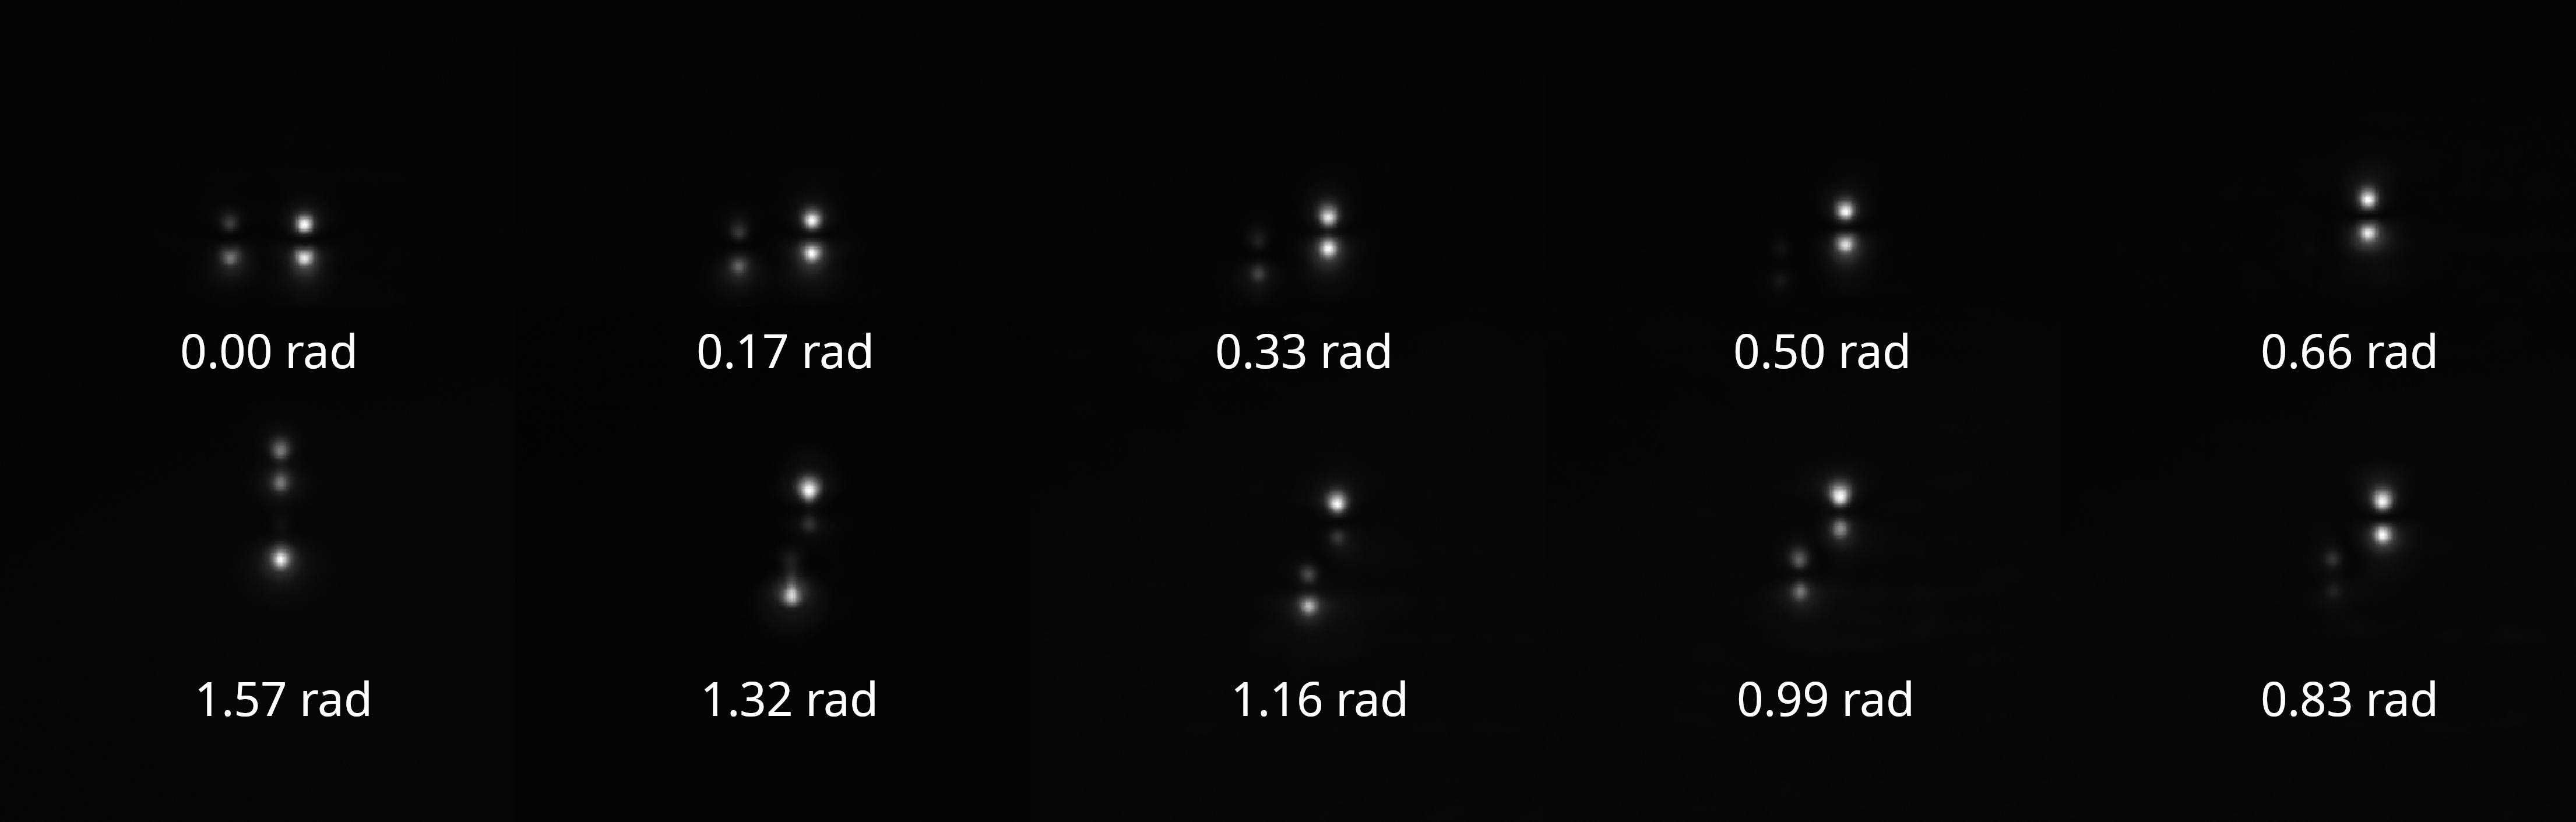
\includegraphics[trim={0 2cm 0 4cm},clip, width=\linewidth]{media/26um_15mm_angles.png}
	\caption{Barrido en ángulo que captura el paso por acoplamiento nulo en ~0.50 rad para una misma distancia de propagación de 15 mm. \label{fig:angulobarrido}}
\end{figure}
Se hizo un análisis de las imágenes como el descrito en la sección \ref{sec:analimag}. Luego, utilizando la descripción discreta (\ref{eqn:CMT_mat}) de la constante de acoplamiento $C = \frac{1}{L}\arctan\left(\sqrt{P_2/P_1}\right)$ se caracterizó su comportameinto en función del ángulo $\theta$ medido desde la horizontal para una distancia de separación fija de 25 $\mu$m. El signo negativo se añadió de manera que la tendencia de los datos fuera continua, como se aprecia en la Figura \ref{fig:coupangle}.
\begin{figure}[H]
\centering
	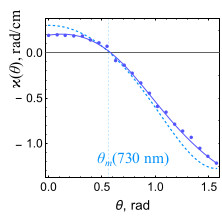
\includegraphics[width=0.5\linewidth]{media/couplingvsangle.jpg}
	\caption{Curva de acomplamiento en función del ángulo entre modos P.\label{fig:coupangle}}
\end{figure}
\section{Redes tipo panal de abeja}
La red tipo panal de abeja es conocida por ser la red subyacente a la estructura del grafeno. Su característica más relevante para efectos de esta tesis tiene relación con sus bandas de Bloch: ambas dispersivas y con la presencia de un cono de Dirac en su intersección \citep{honeycombdirac}.

Una vez encontrados los parámetros de fabricación de la sección anterior, se estudió el mismo efecto en una red tipo panal de abeja de forma que la distancia entre sitios se dejó fija (Figura \ref{fig:HCLBW}). Se hizo un barrido de ángulos para evidenciar el efecto. 
\begin{figure}[H]
\centering
	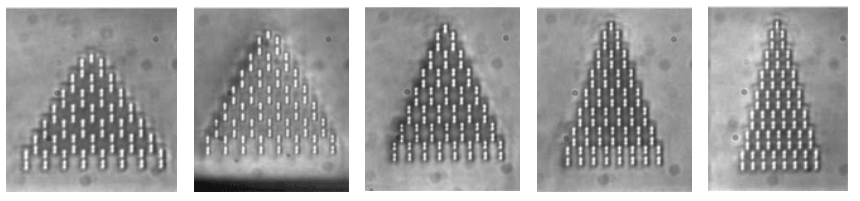
\includegraphics[width=\linewidth]{media/honeycomb_lattices_bw.png}
	\caption{Imágenes microscópicas de redes fotónicas tipo panel de abeja.\label{fig:HCLBW}}
\end{figure}